\question \textbf{HMM probabilities}

An HMM (hidden Markov model) is a probabilistic graphical model with three types of probabilities.

\noindent
Transition probabilities:
\begin{table}[H]
\centering
\begin{tabular}{|c|c|c|}
\hline
     & $\mathrm{L_t}$  & $\mathrm{H_t}$  \\ \hline
$\mathrm{L_{t-1}}$ & 0.2 & 0.8 \\ \hline
$\mathrm{H_{t-1}}$ & 0.4 & 0.6 \\ \hline
\end{tabular}
\end{table}

\noindent
Emission probabilities:
\begin{table}[H]
\centering
\begin{tabular}{|c|c|c|}
\hline
     & L  & H  \\ \hline
Sunny & 0.5 & 0.7 \\ \hline
Rain & 0.5 & 0.3 \\ \hline
\end{tabular}
\end{table}

\noindent
Initial transition probabilities:
\begin{center}
(L, H) = (0.3, 0.7)
\end{center}

\vspace{0.1 in}

\begin{parts}

%% (a)
  \part Add the transition and emission probabilities to the graph.
\begin{figure}[H]
      \centering
      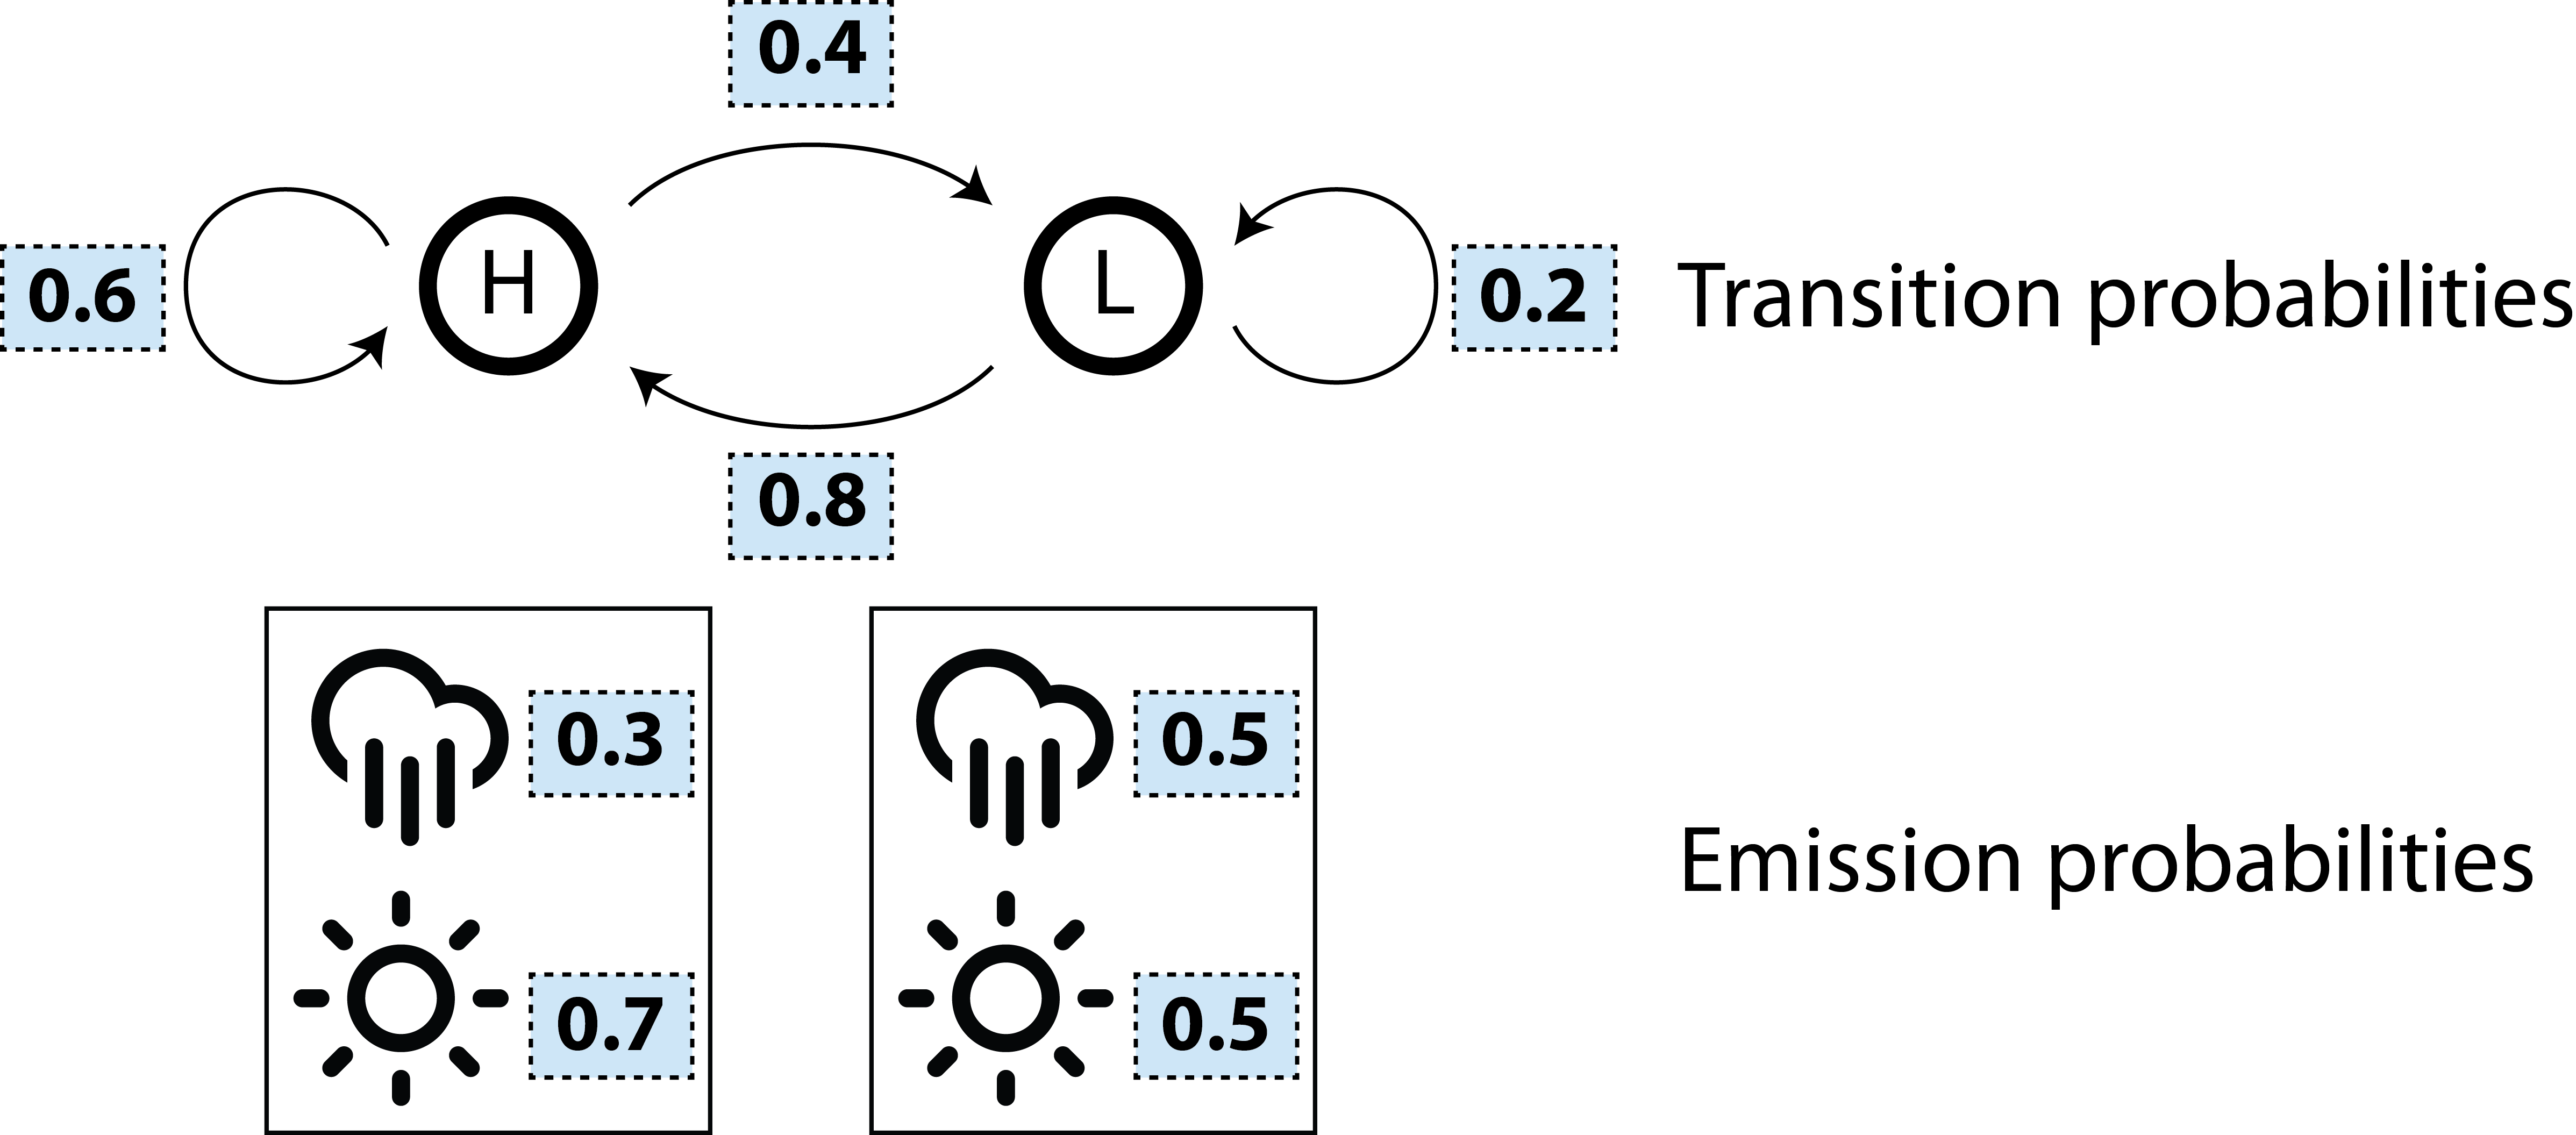
\includegraphics[width=0.6 \textwidth]{fig13/hmm_probabilities_solution.png}
\end{figure}

%% (b)
  \part What are the joint probabilities for (Rain, Rain, Sunny) and (H, L, L)?
\begin{solution}[0.35 in]
p(H)p(Rain$\mid$H) $\times$ p(L$\mid$H)p(Rain$\mid$L) $\times$ p(L$\mid$L)p(Sunny$\mid$L) \\
\null \quad  \quad \quad \quad \quad $= 0.7 \times 0.3 \times 0.4 \times 0.5 \times 0.2 \times 0.5 = 0.0042$
\end{solution}

%% (c)
  \part What are the joint probabilities for (Sunny, Rain, Sunny) and (L, H, L)?
\begin{solution}[0.35 in]
p(L)p(Sunny$\mid$L)  $\times$  p(H$\mid$L)p(Rain$\mid$H) $\times$  p(L$\mid$H)p(Sunny$\mid$L) \\
\null \quad  \quad \quad \quad \quad $= 0.3 \times 0.5 \times 0.8 \times 0.3  \times 0.4 \times 0.5 = 0.0072$
\end{solution}

\end{parts}
